\begin{figure}[t]
    \centering
    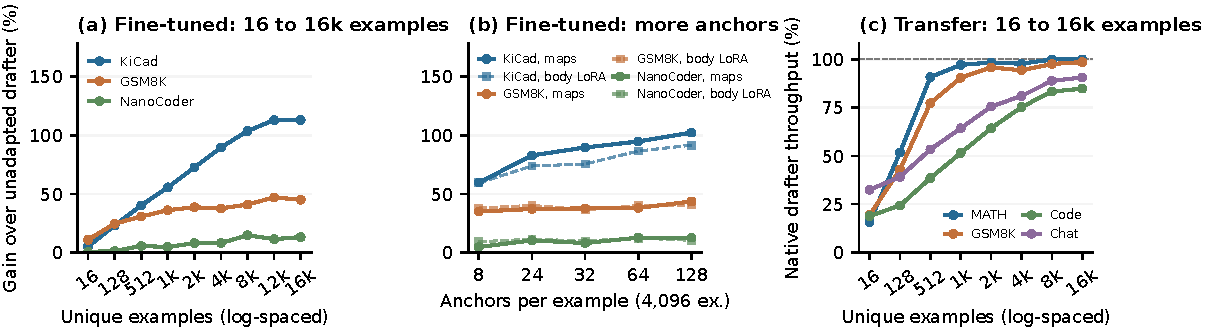
\includegraphics[width=\linewidth]{figures/relayspec_scaling.pdf}
    \caption{Supervision budget in both settings, from 16 to 16{,}384 training examples. (a) and (c) share a log-spaced example axis; (b) fixes examples at 4{,}096 and varies anchors per example. (a) and (b) use fine-tuned Qwen3-4B targets with the accept-until-fail objective, where solid lines train the five interface maps and dashed lines train a rank-128 LoRA inside the draft transformer. (c) transfers the Qwen3-4B drafter to Qwen3-8B with the reconstruction objective and plots throughput as a percentage of the native Qwen3-8B drafter. Adaptation is already effective at 16 examples and speedup keeps improving with supervision without saturating at the largest budget measured.}
    \label{fig:scaling}
\end{figure}
